\subsection{Numerical reconstruction of the nonequilibrium steady-state density}
\label{sec:three_mode_ness_density}

We numerically reconstruct the stationary density of the driven three-mode
system in the full reduced state
\(x=(I_1,I_2,I_3,\theta_1,\theta_3)\), with respect to the measure
\(\mathrm dI_1\mathrm dI_2\mathrm dI_3\mathrm d\theta_1\mathrm d\theta_3\).
The baths are fixed at \((T_1,T_3)=(2,8)\) and \(\gamma=0.1\).  Rather than
learning an unconstrained density, we write
\begin{equation}
 \rho_m(x)=\frac{1}{Z_{\rm eq}Z_m}
 \exp\!\left[-\frac{E(x)}{5}+f_m(x)\right],
 \qquad
 \widehat\rho_{\rm ss}(x)=\frac{1}{3}\sum_{m=1}^{3}\rho_m(x),
 \label{eq:ness_density_ratio}
\end{equation}
where the equilibrium Gibbs factor provides the exact boundary decay and the
neural correction \(f_m\) represents the nonequilibrium distortion.  The three
members use independent training seeds.  Their normalizers \(Z_m\) are
estimated on independent equilibrium-reference trajectories, while direct
integration of the Gibbs factor gives
\(Z_{\rm eq}=514.3433631\) (standard error \(1.14\times10^{-5}\)).

The correction is a two-hidden-layer, 128-unit tanh network acting on smooth
log-action, periodic angular, and explicit bond-transport features.  Training
combines the stationary Fokker--Planck residual with moment constraints.  The
fixed neural output is calibrated by the same three-observable exponential
tilt at both timesteps, using \(I_1\), \(I_1I_2\sin\theta_1\), and
\(I_2I_3\sin\theta_3\), with a frozen 0.625 shrink factor.  We
split data by complete trajectories, not individual snapshots.  The final
fine-step assessment uses a fresh 64-stream holdout at
\(\Delta t=2.5\times10^{-4}\), divided into 32 validation and 32 test streams;
each stream contains 100001 stationary snapshots after burn-in.  All selection
decisions and diagnostic thresholds were frozen before the corresponding test
split was opened.

On the independent fine-step test, all three models pass the preregistered
criteria.  The effective-sample fractions are 0.9156--0.9173, the median
absolute relative stationary-equation residuals are 0.08869--0.09548, the
largest of the twelve stream-bootstrap moment discrepancies is
\(1.45\) standard errors, and the largest marginal total-variation distance is
0.0244.  The maximum pairwise centered log-density-ratio RMS is 0.0127.  The
same pipeline applied at equilibrium, where the exact correction is
\(f=0\), also passes both validation and test.

\begin{figure}[!htbp]
 \centering
 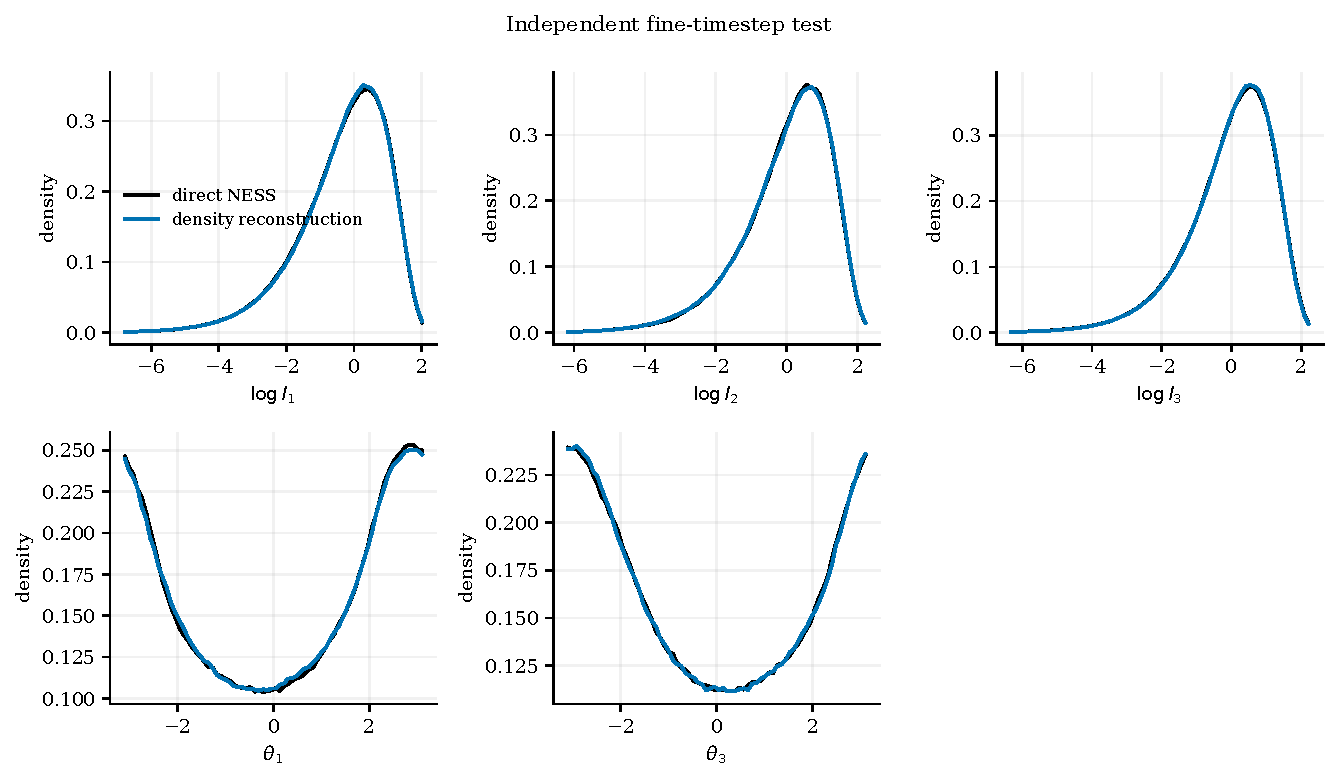
\includegraphics[width=\linewidth]{final_figures/ness_marginals_fine.pdf}
 \caption{Held-out fine-step marginals.  Direct stationary histograms (black)
 are compared with marginals reconstructed from the normalized five-dimensional
 density (blue).  The blue band spans the three independently trained models.}
 \label{fig:ness_density_marginals}
\end{figure}

The reconstruction is not merely a collection of one-dimensional marginals.
Figure~\ref{fig:ness_density_angles} compares the directly sampled joint
angular distribution with the corresponding marginal of
\(\widehat\rho_{\rm ss}\).  The residual panel contains no coherent missing
structure at the resolved scale.  Slices of the absolute density at fixed
actions, Fig.~\ref{fig:ness_density_slices}, expose the changing phase geometry
as the action level increases.

\begin{figure}[!htbp]
 \centering
 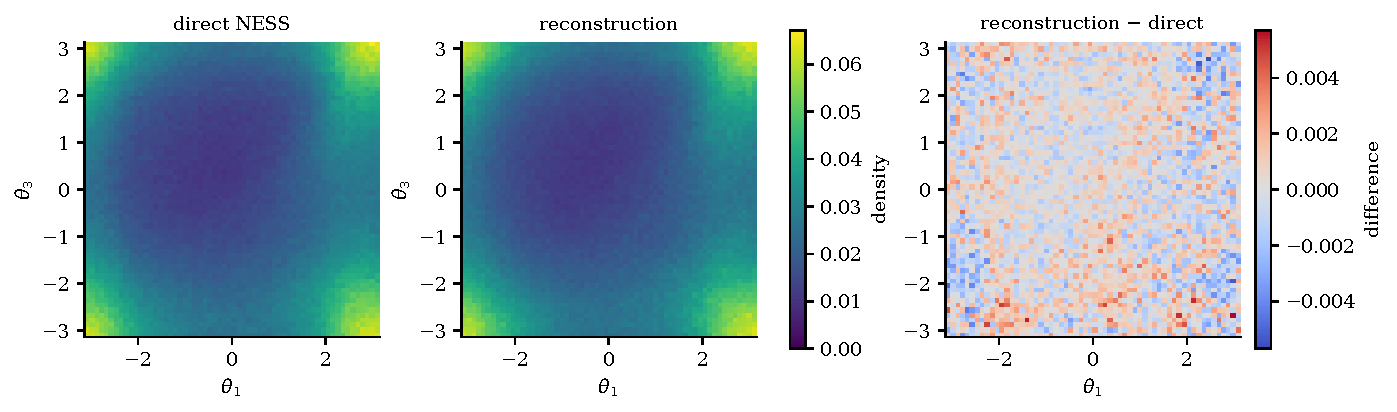
\includegraphics[width=\linewidth]{final_figures/ness_angle_joint_fine.pdf}
 \caption{Joint angular marginal on the independent fine-step test: direct
 NESS sample, density reconstruction, and their difference.}
 \label{fig:ness_density_angles}
\end{figure}

\begin{figure}[!htbp]
 \centering
 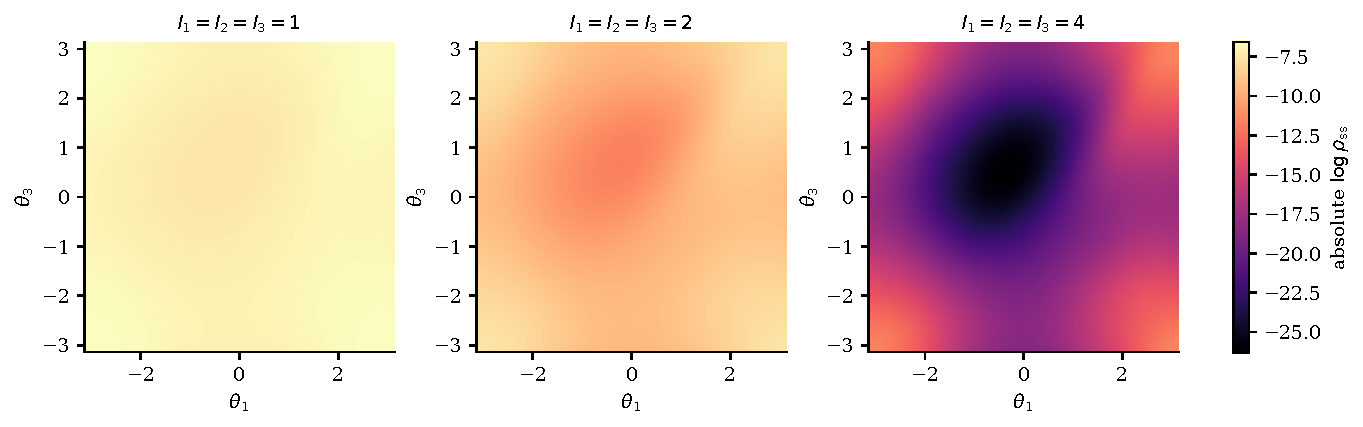
\includegraphics[width=\linewidth]{final_figures/ness_density_angle_slices.pdf}
 \caption{Absolute log-density slices of Eq.~\eqref{eq:ness_density_ratio} at
 equal actions \(I_1=I_2=I_3\in\{1,2,4\}\).  A common color scale is used.}
 \label{fig:ness_density_slices}
\end{figure}

We finally repeat the complete inference at \(\Delta t=10^{-3}\).  The first
coarse model failed validation because one right-bond transport moment reached
\(|z|=3.963\), above the frozen 3.748 threshold; that failure was retained.
A separately frozen recovery added this right-current moment to the exponential
calibration, without changing the neural weights or inspecting the coarse test.
The recovered estimator then passed validation and its one-shot test.  On the
coarse test its ESS is 0.9087--0.9114, residual median is 0.08943--0.09310,
maximum moment discrepancy is 2.83 standard errors, and maximum marginal TV is
0.0242.  We subsequently applied that same three-moment procedure to the fine
model without retraining and declared one final test access before validation.
It passed every gate and changed the fine ensemble centered log density by only
0.00152 RMS.  More importantly, the resulting three-moment-to-three-moment
fine/coarse ensemble log-density RMS is 0.02436 on the fine support and 0.02435
on the coarse support, well below
the predeclared 0.10 replication threshold.

These tests support treating \(\widehat\rho_{\rm ss}\) as a numerical solution
of the full reduced five-dimensional NESS on the stationary region sampled by
the trajectories.  The qualification is essential: this is not a closed-form
global solution, and the accuracy of the learned correction has not been
established in extreme, unsampled low-density tails.
